\documentclass[border=10pt]{standalone}
\usepackage{tikz}
\usetikzlibrary{arrows.meta, positioning, calc, fit, backgrounds, decorations.pathreplacing}

\begin{document}
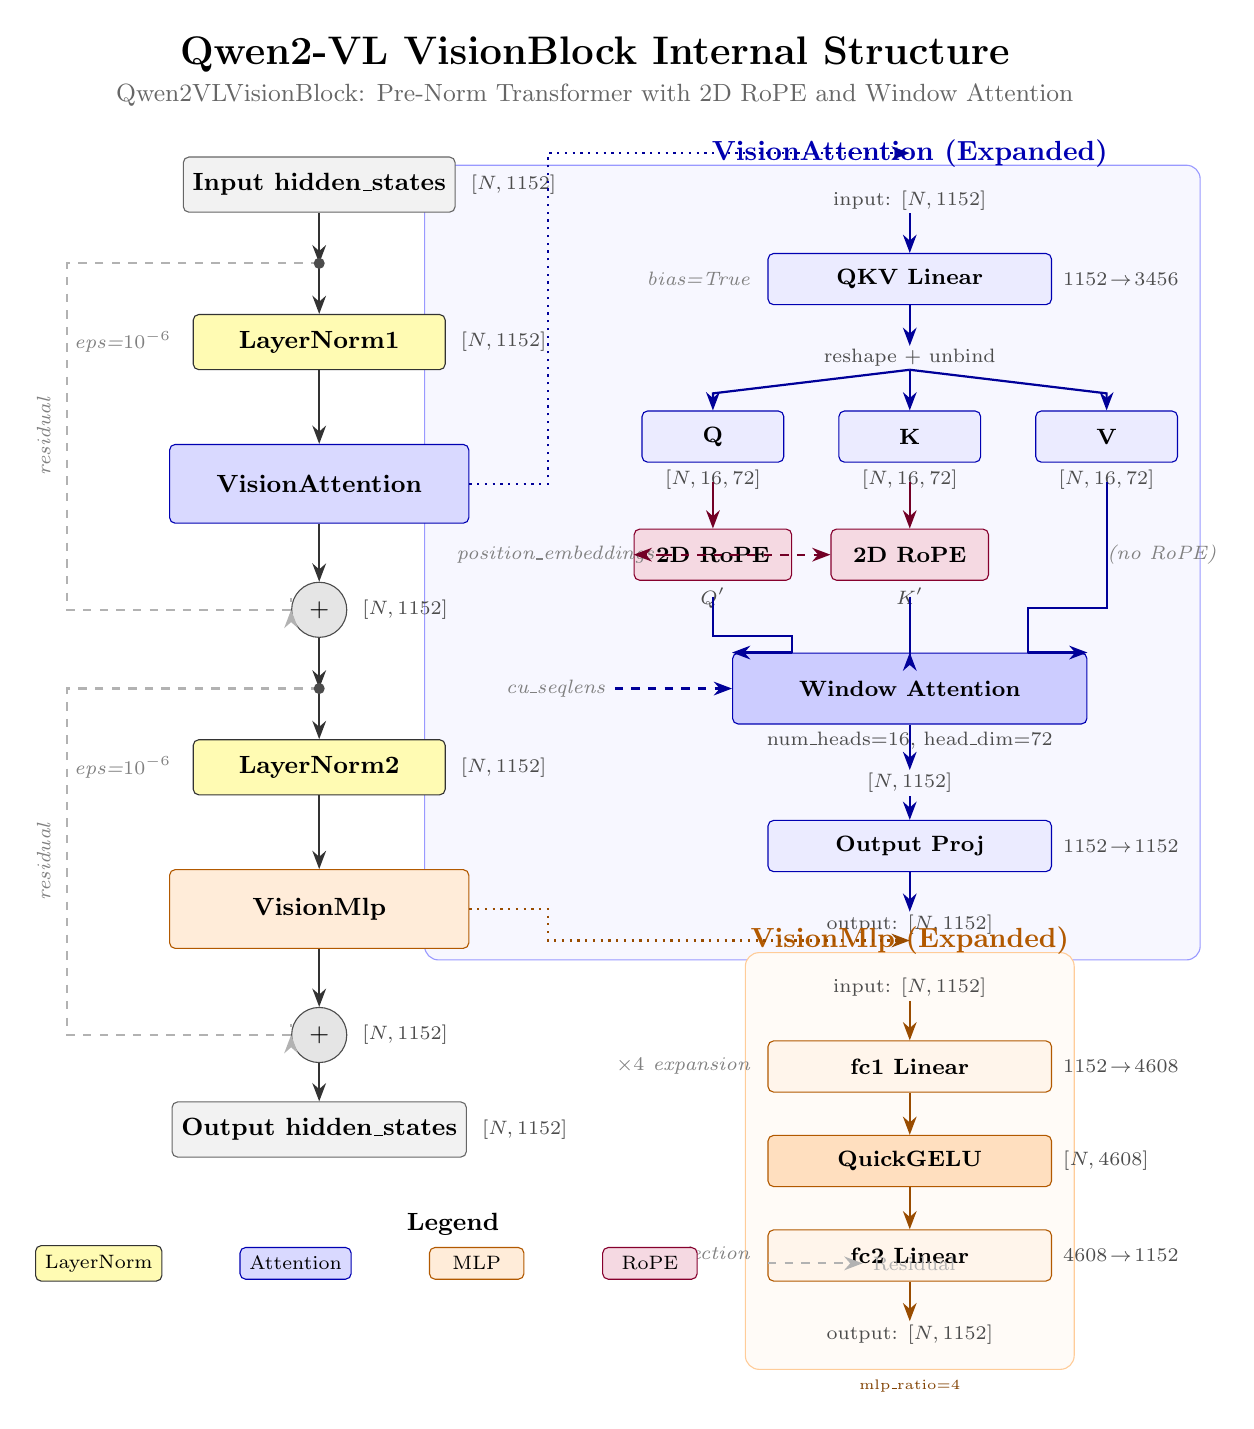
\begin{tikzpicture}[
    >=Stealth,
    node distance=1.2cm,
    % Box styles
    normbox/.style={rectangle, draw=black!80, fill=yellow!30, minimum width=3.2cm, minimum height=0.7cm, font=\small\bfseries, rounded corners=2pt},
    attnbox/.style={rectangle, draw=blue!70!black, fill=blue!15, minimum width=3.2cm, minimum height=0.7cm, font=\small\bfseries, rounded corners=2pt},
    attndetail/.style={rectangle, draw=blue!70!black, fill=blue!8, minimum width=2.4cm, minimum height=0.65cm, font=\footnotesize\bfseries, rounded corners=2pt},
    mlpbox/.style={rectangle, draw=orange!70!black, fill=orange!15, minimum width=3.2cm, minimum height=0.7cm, font=\small\bfseries, rounded corners=2pt},
    mlpdetail/.style={rectangle, draw=orange!70!black, fill=orange!8, minimum width=2.4cm, minimum height=0.65cm, font=\footnotesize\bfseries, rounded corners=2pt},
    ropebox/.style={rectangle, draw=purple!70!black, fill=purple!15, minimum width=2.0cm, minimum height=0.65cm, font=\footnotesize\bfseries, rounded corners=2pt},
    addbox/.style={circle, draw=black!70, fill=gray!20, minimum size=0.7cm, font=\small\bfseries},
    iobox/.style={rectangle, draw=black!60, fill=gray!10, minimum width=3.2cm, minimum height=0.7cm, font=\small\bfseries, rounded corners=2pt},
    dimlab/.style={font=\scriptsize\color{black!70}, inner sep=1pt},
    arrmain/.style={->, thick, black!80},
    arrblue/.style={->, thick, blue!60!black},
    arrorange/.style={->, thick, orange!60!black},
    arrpurple/.style={->, thick, purple!60!black},
    arrgray/.style={->, thick, gray!60, dashed},
    sidelabel/.style={font=\scriptsize\itshape\color{black!50}},
]

% ============================================================
% MAIN DATA PATH (left column, x=0)
% ============================================================

% Input
\node[iobox] (input) at (0, 0) {Input hidden\_states};
\node[dimlab, right=0.15cm of input] {$[N, 1152]$};

% Fork point 1
\coordinate (fork1) at (0, -1.0);

% LayerNorm 1
\node[normbox] (norm1) at (0, -2.0) {LayerNorm1};
\node[dimlab, right=0.15cm of norm1] {$[N, 1152]$};
\node[sidelabel, left=0.15cm of norm1] {eps=$10^{-6}$};

% Attention block placeholder (main path shows the box)
\node[attnbox, minimum height=1.0cm, minimum width=3.8cm] (attn_main) at (0, -3.8) {VisionAttention};

% Add 1
\node[addbox] (add1) at (0, -5.4) {$+$};
\node[dimlab, right=0.15cm of add1] {$[N, 1152]$};

% Fork point 2
\coordinate (fork2) at (0, -6.4);

% LayerNorm 2
\node[normbox] (norm2) at (0, -7.4) {LayerNorm2};
\node[dimlab, right=0.15cm of norm2] {$[N, 1152]$};
\node[sidelabel, left=0.15cm of norm2] {eps=$10^{-6}$};

% MLP block placeholder
\node[mlpbox, minimum height=1.0cm, minimum width=3.8cm] (mlp_main) at (0, -9.2) {VisionMlp};

% Add 2
\node[addbox] (add2) at (0, -10.8) {$+$};
\node[dimlab, right=0.15cm of add2] {$[N, 1152]$};

% Output
\node[iobox] (output) at (0, -12.0) {Output hidden\_states};
\node[dimlab, right=0.15cm of output] {$[N, 1152]$};

% --- Main path arrows ---
\draw[arrmain] (input.south) -- (fork1);
\draw[arrmain] (fork1) -- (norm1.north);
\draw[arrmain] (norm1.south) -- (attn_main.north);
\draw[arrmain] (attn_main.south) -- (add1.north);
\draw[arrmain] (add1.south) -- (fork2);
\draw[arrmain] (fork2) -- (norm2.north);
\draw[arrmain] (norm2.south) -- (mlp_main.north);
\draw[arrmain] (mlp_main.south) -- (add2.north);
\draw[arrmain] (add2.south) -- (output.north);

% --- Residual connections (gray dashed) ---
% Residual 1: fork before norm1, join at add1
\draw[arrgray] (fork1) -| (-3.2, -1.0) -- (-3.2, -5.4) -| (add1.west);
\node[sidelabel] at (-3.5, -3.2) {\rotatebox{90}{residual}};

% Residual 2: fork before norm2, join at add2
\draw[arrgray] (fork2) -| (-3.2, -6.4) -- (-3.2, -10.8) -| (add2.west);
\node[sidelabel] at (-3.5, -8.6) {\rotatebox{90}{residual}};

% Small dots at fork points
\fill[black!70] (fork1) circle (2pt);
\fill[black!70] (fork2) circle (2pt);


% ============================================================
% EXPANDED ATTENTION DETAIL (right column, x=7)
% ============================================================

\begin{scope}[shift={(7.5, -0.2)}]

    % Title
    \node[font=\normalsize\bfseries, blue!70!black] at (0, 0.6) {VisionAttention (Expanded)};
    
    % Input from norm1
    \node[dimlab] (attn_in) at (0, 0) {input: $[N, 1152]$};
    
    % QKV Linear
    \node[attndetail, minimum width=3.6cm] (qkv) at (0, -1.0) {QKV Linear};
    \node[dimlab, right=0.1cm of qkv] {$1152 \!\to\! 3456$};
    \node[sidelabel, left=0.1cm of qkv] {bias=True};
    
    % Split into Q, K, V
    \node[dimlab] (split_label) at (0, -2.0) {reshape + unbind};
    
    \node[attndetail, minimum width=1.8cm] (qhead) at (-2.5, -3.0) {Q};
    \node[dimlab, below=0.05cm of qhead] {$[N, 16, 72]$};
    
    \node[attndetail, minimum width=1.8cm] (khead) at (0, -3.0) {K};
    \node[dimlab, below=0.05cm of khead] {$[N, 16, 72]$};
    
    \node[attndetail, minimum width=1.8cm] (vhead) at (2.5, -3.0) {V};
    \node[dimlab, below=0.05cm of vhead] {$[N, 16, 72]$};
    
    % RoPE on Q and K
    \node[ropebox] (rope_q) at (-2.5, -4.5) {2D RoPE};
    \node[ropebox] (rope_k) at (0, -4.5) {2D RoPE};
    
    \node[dimlab, below=0.05cm of rope_q] {$Q'$};
    \node[dimlab, below=0.05cm of rope_k] {$K'$};
    
    % Position embeddings input
    \node[sidelabel] (posemb) at (-4.5, -4.5) {position\_embeddings};
    \draw[arrpurple, dashed] (posemb.east) -- (rope_q.west);
    \draw[arrpurple, dashed] (posemb.east) -- ++(0.5,0) |- (rope_k.west);
    
    % Window Attention
    \node[attndetail, minimum width=4.5cm, minimum height=0.9cm, fill=blue!20] (winattn) at (0, -6.2) {Window Attention};
    \node[dimlab, below=0.05cm of winattn] {num\_heads=16, head\_dim=72};
    
    % cu_seqlens input
    \node[sidelabel] (cuseq) at (-4.5, -6.2) {cu\_seqlens};
    \draw[arrblue, dashed] (cuseq.east) -- (winattn.west);
    
    % Attention output
    \node[dimlab] (attn_out_dim) at (0, -7.4) {$[N, 1152]$};
    
    % Output Projection
    \node[attndetail, minimum width=3.6cm] (proj) at (0, -8.2) {Output Proj};
    \node[dimlab, right=0.1cm of proj] {$1152 \!\to\! 1152$};
    
    % Attention output
    \node[dimlab] (attn_final) at (0, -9.2) {output: $[N, 1152]$};
    
    % --- Attention internal arrows ---
    \draw[arrblue] (attn_in.south) -- (qkv.north);
    \draw[arrblue] (qkv.south) -- (split_label.north);
    
    % Split arrows
    \draw[arrblue] (split_label.south) -- ++(-2.5, -0.3) -- (qhead.north);
    \draw[arrblue] (split_label.south) -- (khead.north);
    \draw[arrblue] (split_label.south) -- ++(2.5, -0.3) -- (vhead.north);
    
    % Q -> RoPE, K -> RoPE
    \draw[arrpurple] (qhead.south) ++(0, -0.25) -- (rope_q.north);
    \draw[arrpurple] (khead.south) ++(0, -0.25) -- (rope_k.north);
    
    % Q', K', V -> Window Attention
    \draw[arrblue] (rope_q.south) ++(0, -0.2) -- ++(0, -0.5) -| (-1.5, -5.75) -- (-1.5, -5.75) |- (winattn.north west);
    \draw[arrblue] (rope_k.south) ++(0, -0.2) -- (0, -5.75) -- (winattn.north);
    \draw[arrblue] (vhead.south) ++(0, -0.25) -- ++(0, -1.6) -| (1.5, -5.75) |- (winattn.north east);
    
    % V bypass (no RoPE)
    \node[sidelabel] at (3.2, -4.5) {(no RoPE)};
    
    % Window attn -> proj
    \draw[arrblue] (winattn.south) -- (attn_out_dim.north);
    \draw[arrblue] (attn_out_dim.south) -- (proj.north);
    \draw[arrblue] (proj.south) -- (attn_final.north);
    
    % Bounding box
    \begin{pgfonlayer}{background}
        \node[draw=blue!40, fill=blue!3, rounded corners=5pt, 
              fit=(attn_in)(qkv)(qhead)(vhead)(rope_q)(rope_k)(winattn)(proj)(attn_final)(posemb)(cuseq),
              inner sep=8pt] (attn_bound) {};
    \end{pgfonlayer}
    
\end{scope}


% ============================================================
% EXPANDED MLP DETAIL (right column, x=7, below attention)
% ============================================================

\begin{scope}[shift={(7.5, -10.2)}]

    % Title
    \node[font=\normalsize\bfseries, orange!70!black] at (0, 0.6) {VisionMlp (Expanded)};
    
    % Input
    \node[dimlab] (mlp_in) at (0, 0) {input: $[N, 1152]$};
    
    % fc1
    \node[mlpdetail, minimum width=3.6cm] (fc1) at (0, -1.0) {fc1 Linear};
    \node[dimlab, right=0.1cm of fc1] {$1152 \!\to\! 4608$};
    \node[sidelabel, left=0.1cm of fc1] {$\times 4$ expansion};
    
    % QuickGELU
    \node[mlpdetail, minimum width=3.6cm, fill=orange!25] (gelu) at (0, -2.2) {QuickGELU};
    \node[dimlab, right=0.1cm of gelu] {$[N, 4608]$};
    
    % fc2
    \node[mlpdetail, minimum width=3.6cm] (fc2) at (0, -3.4) {fc2 Linear};
    \node[dimlab, right=0.1cm of fc2] {$4608 \!\to\! 1152$};
    \node[sidelabel, left=0.1cm of fc2] {projection};
    
    % Output
    \node[dimlab] (mlp_out) at (0, -4.4) {output: $[N, 1152]$};
    
    % --- MLP internal arrows ---
    \draw[arrorange] (mlp_in.south) -- (fc1.north);
    \draw[arrorange] (fc1.south) -- (gelu.north);
    \draw[arrorange] (gelu.south) -- (fc2.north);
    \draw[arrorange] (fc2.south) -- (mlp_out.north);
    
    % Bounding box
    \begin{pgfonlayer}{background}
        \node[draw=orange!40, fill=orange!3, rounded corners=5pt,
              fit=(mlp_in)(fc1)(gelu)(fc2)(mlp_out),
              inner sep=8pt, label={[font=\tiny\color{orange!50!black}]below:mlp\_ratio=4}] (mlp_bound) {};
    \end{pgfonlayer}
    
\end{scope}


% ============================================================
% CONNECTION ARROWS (main -> expanded)
% ============================================================

% Attention: main block -> expanded detail
\draw[arrblue, thick, dotted] (attn_main.east) -- ++(1.0, 0) |- (7.5, 0.4) node[midway, above, font=\scriptsize\color{blue!60!black}] {};

% MLP: main block -> expanded detail
\draw[arrorange, thick, dotted] (mlp_main.east) -- ++(1.0, 0) |- (7.5, -9.6) node[midway, above, font=\scriptsize\color{orange!60!black}] {};


% ============================================================
% TITLE
% ============================================================

\node[font=\Large\bfseries, anchor=north] at (3.5, 2.0) {Qwen2-VL VisionBlock Internal Structure};
\node[font=\small\color{black!60}, anchor=north] at (3.5, 1.4) {Qwen2VLVisionBlock: Pre-Norm Transformer with 2D RoPE and Window Attention};


% ============================================================
% LEGEND
% ============================================================

\begin{scope}[shift={(-3.8, -13.5)}]
    \node[font=\small\bfseries] at (5.5, 0.3) {Legend};
    
    \node[rectangle, draw=black!80, fill=yellow!30, minimum width=1.2cm, minimum height=0.4cm, rounded corners=2pt, font=\scriptsize] at (1.0, -0.2) {LayerNorm};
    \node[rectangle, draw=blue!70!black, fill=blue!15, minimum width=1.2cm, minimum height=0.4cm, rounded corners=2pt, font=\scriptsize] at (3.5, -0.2) {Attention};
    \node[rectangle, draw=orange!70!black, fill=orange!15, minimum width=1.2cm, minimum height=0.4cm, rounded corners=2pt, font=\scriptsize] at (5.8, -0.2) {MLP};
    \node[rectangle, draw=purple!70!black, fill=purple!15, minimum width=1.2cm, minimum height=0.4cm, rounded corners=2pt, font=\scriptsize] at (8.0, -0.2) {RoPE};
    \draw[arrgray] (9.5, -0.2) -- ++(1.2, 0) node[right, font=\scriptsize] {Residual};
\end{scope}

\end{tikzpicture}
\end{document}
